\documentclass{article}
\usepackage{amsfonts, amsmath, amssymb, amsthm, graphicx} % Math 
\graphicspath{ {./../images} }
\usepackage{enumitem}
\setlength{\parindent}{0pt} \oddsidemargin -0.2in \evensidemargin
0.0in \topmargin -1in \textheight 9.9in \textwidth 6.9in

\newtheorem{thm}{Theorem}
\newtheorem{prop}[thm]{Proposition}
\newtheorem{cor}[thm]{Corollary}

\newenvironment{problem}[2][Question]{\begin{trivlist}
\item[\hskip \labelsep {\bfseries #1}\hskip \labelsep {\bfseries #2.}]}{\end{trivlist}}

% main content
\begin{document} 

\textbf{Math 158 HW1}

% Q1.7.2
\begin{problem}{1}
    Let $K_{n:r}$ denote the Kneser graph, whose vertex set is the set of
    r-element subsets of an n-element set, and where two vertices form an edge if the
    corresponding sets are disjoint.
    \begin{enumerate}[label=(\alph*)]
    \item Describe $K_{n:1}$ for $n \geq 1$.
    \begin{proof}[Solution]
        Since $\forall v,u \in V(K_{n:1})$, $v \cap u = \emptyset$. Thus, $\forall v,u \in V(K_{n:1})$, $\{v, u\} \in E(K_{n:1})$, which makes $K_{n:1}$ a $K_n$ complete graph.
    \end{proof}
    
    \item Draw $K_{4:2}$ and $K_{5:2}$.
    \begin{proof}[Solution]
        Graphs of $K_{4:2}$ and $K_{5:2}$: \\
        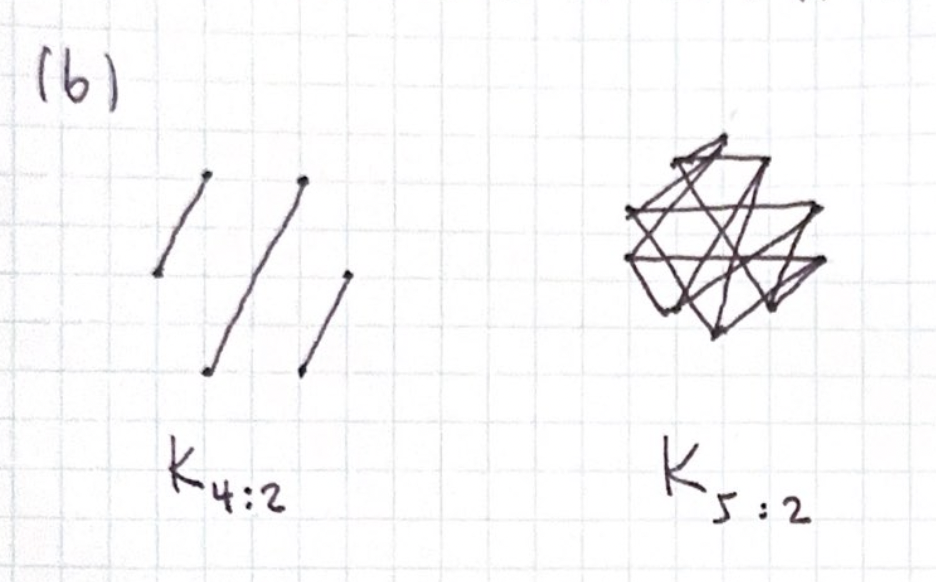
\includegraphics[width=\textwidth]{Q172b}
    \end{proof}

    \item Determine $|E({K_{n:r}})|$ for $n \geq 2r \geq 1$.
    
    \begin{proof}[Solution]
        For each $v \in V(K_{n:r}$, $v$ forms edges with other vertices whose vertex set is $r$ of the other $n-r$ elements that are not in the vertex set of $v$, which implies that $d_{K_{n:r}}(v) = {{n-r} \choose {r}}$. Since there are $n \choose r$ vertices in $K_{n:r}$, by the Handshake Theorem, we have  $|E(K_{n:r})| = \binom{n}{r}\binom{n-r}{r}/2$.
    \end{proof}
\end{enumerate}
\end{problem}

\newpage

% Q1.7.4
\begin{problem}{2}
    Let $G$ be a digraph such that every vertex has a positive in-degree. Prove that $G$ contains a directed cycle.
\end{problem}
\begin{proof}
    We will prove this by contradiction. Let $v \in V(G)$.  Suppose for the sake of contradiction that $G$ does not contain any directed cycle. Starting from $v$, we can find a path $P$ by tracing back to a vertex with an edge directed to the current vertex we're on. We then add the vertex to $P$ and go to that vertex, and we repeat the previous actions. Since every vertex in $G$ has a positive in-degree, we can always find another vertex that has a directed edge to the current vertex we're on and not in $P$. However, this makes $G$ have infinitely many vertices, which is a contradiction. Therefore, $G$ contains a directed cycle.
\end{proof}

\newpage

% Q1.7.12
\begin{problem}{3}
 Let $g$ be an n-vertex graph with $n \geq 2$ and $\delta(G) \geq (n-1)/2$. Prove that $G$ is connected and the diameter of $G$ is at most two.
\end{problem}
\begin{proof}
    We will first prove that $G$ is connected by contradiction. Suppose for the sake of contradiction that $G$ is disconnected. Let $n = |V(G)|$, $v \in V(G)$, $H$ be the component of $G$ that contains $v$. Since $d_G(v) \geq \delta(G) \geq (n-1)/2$, we have $|V(H)| \geq (n-1)/2 + 1 = (n+1)/2$, which implies that other components in $G$ contain at most $n - (n+1)/2 = (n-1)/2$ vertices. However, this shows that $\Delta(G-V(H)) \leq (n-1)/2 - 1 < (n-1)/2$, which contradicts $\delta(G) \geq (n-1)/2$ because $H$ is disconnected to $G-V(H)$. Therefore, $G$ is connected.

    We will now prove that the diameter of $G$ is at most two. Let $u, w \in V(G)$. If $u \in N(w)$, then $d_G(u, w) = 1$. If $u \notin N(w)$, then $N(u), N(w) \in V(G) \backslash \{u, w\}$. Since $|N(u)|, |N(w)| \geq \delta(G) \geq (n-1)/2$, we have $|N(u)| + |N(w)| > n - 2 = |V(G) \backslash \{u, w\}|$. Hence, $|N(u)| \cap |N(w)| \neq \emptyset$, which means that $d_G(u, w) = 2$. Therefore, the diameter of $G$ is at most two.
\end{proof}

\newpage

% Q1.7.14.a
\begin{problem}{4}
     Let $P$ and $Q$ be the longest paths in a connected graph $G$. Prove that
     \[V(P) \cap V(Q) \neq \emptyset.\]
\end{problem}
\begin{proof}
    We will prove this by contradiction. Let $P, Q$ be the longest paths in a connected graph $G$, with $\{p_1, p_2, \dots, p_{n+1}\}$ and $\{q_1, q_2, \dots, q_{n+1}\}$ as their vertex sets respectively, and $n = |E(P)| = |E(Q)|$.  Suppose for the sake of contradiction that $V(P) \cap V(Q) = \emptyset$. Since $G$ is connected, there must be a path $R$ that starts from $p_i$ and ends at $q_j$, for some $1 \leq i, j \leq n + 1$. Let $m = d_G(p_i, q_j)$. Since $p_i \neq q_j$, we have $m \geq 1$. Let $P'$ be the longer path between $p_1p_2\dots p_i$ and $p_ip_{i+1}\dots p_{n+1}$, $Q'$ be the longer path between $q_1q_2\dots q_j$ and $q_jq_{j+1}\dots q_{n+1}$. By connecting $P'$, $Q'$, and $R$, we get a new path $S$. Since $|E(P')|, |E(Q')| \geq n/2$, $|E(R)| = m \geq 1$, we have $|E(S)| \geq n + 1$, which contradicts that $P, Q$ are the longest paths on $G$.
    Therefore, if $P, Q$ are the longest paths in a connected graph, then $V(P) \cap V(Q) \neq \emptyset$.
\end{proof}

\newpage

% Q2.5.7
\begin{problem}{5}
    Prove that a graph $G$ of minimum degree at least $k \geq 2$ containing no triangles contains a cycle of length at least $2k$.
\end{problem}
\begin{proof}
    Let $P$ be the longest path in $G$, say $v_1v_2\dots v_t$. Then $N(v_1) \subseteq V(P)$ or else we get a longer path. Since $G$ does not contain any triangles, if $v_p, v_q \in N(v_1)$ for some $p > q$, then $p - q \geq 2$. Since $|N(v_1)| \geq \delta(G) \geq k$ and $d_P(v_p, v_q) \geq 2$ for all $v_p, v_q \in N(v_1)$, $t \geq 2k$ and $v_1$ has a neighbor $v_i$ for some $i \geq 2k$. Then, the cycle $v_1 v_2 \dots v_i v_1$ has length at least $2k$.
\end{proof}

\end{document}